\chapter{Appendix}\label{ch:appendix}

\section*{Appendix B: Blackbody Function}

Even at an undergraduate level, we're all fairly familiar with \emph{blackbody radiation}. The easiest way to deduce the expression for the energy density of photons in \emph{thermal equilibrium} (STE) inside a cavity is by the means of statistical mechanics.
\par Remember the Bose-Einstein distribution ($\mu = 0$)
\begin{equation*}
	n = \frac{1}{\exp(h\nu/kT)-1}
\end{equation*}
and the phase space density of states (per unit volume)
\begin{equation*}
	\rho(\nu)\,\text{d}\nu = \frac{4\pi h g \nu^{3}}{c^{3}}\,\text{d}\nu
\end{equation*}
from which deducing the expression from internal energy is straightforward. Remembering $g=2$ is the quantum degeneracy of photons, a simple moltiplication of the previous expressions yields
\begin{equation}
	U_{\nu}\,\text{d}\nu = \frac{8\pi h}{c^{3}}\frac{\nu^{3}}{\exp(h\nu/kT)-1}\,\text{d}\nu
    \label{eq:blackbody_endens}
\end{equation}
\par The energy of a photon is $E_{\gamma} = h\nu$, meaning the number of photons in the frequency range $\nu \to \nu + \text{d}\nu$ is
\begin{equation}
    n_{\nu}\,\text{d}\nu = \frac{8\pi}{c^{3}}\frac{\nu^{2}}{\exp(h\nu/kT)-1}\,\text{d}\nu
    \label{eq:blackbody_numdens}
\end{equation}
which can be integrated over all frequencies, thus obtaining the number density of photons in blackbody radiation
\begin{equation}
    n_{\gamma} = \beta T^{3} \quad \beta = \frac{2.4041 k^{3}}{\pi^{2}\hbar^{3}c^{3}}
    \label{eq:blackbody_totnum}
\end{equation}
\par Since blackbody radiation is isotropic (it depends only on the absolute temperature $T$), the definition of mean monochromatic intensity yields
\begin{equation}
	\boxed{
	B_{\nu}(T) = \frac{2h\nu^{3}}{c^{2}}\frac{1}{\exp(h\nu/kT)-1}
	}
	\label{eq:blackbodyintensity}
\end{equation}
\begin{figure}[h!]
	\centering
	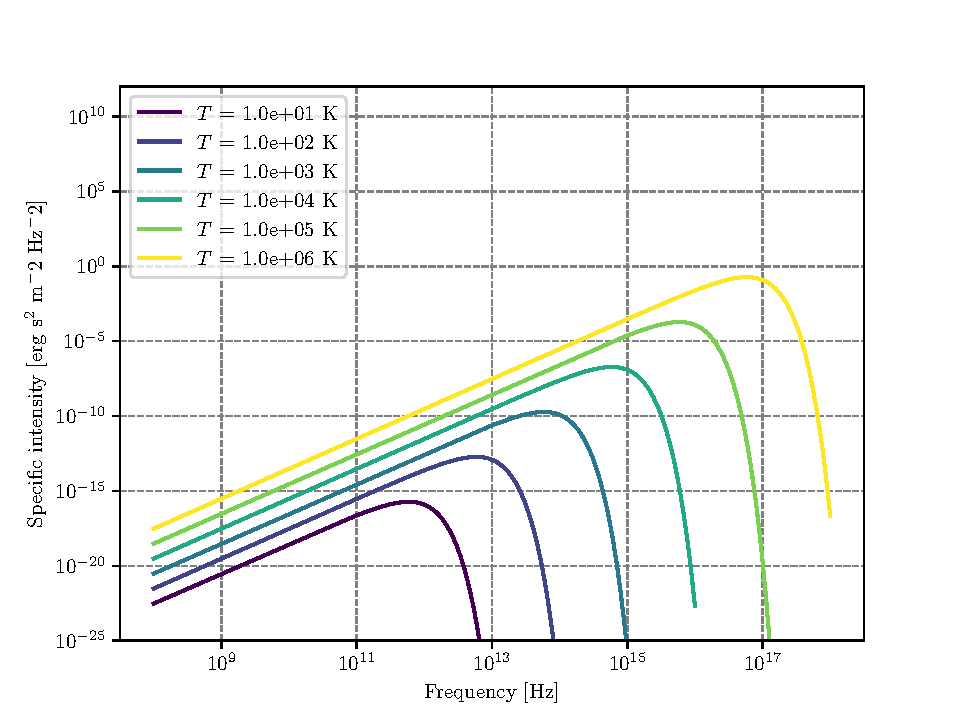
\includegraphics[width=0.9\textwidth]{img/blackbody.pdf}
	\caption{Blackbody frequency spectrum.}
    \label{fgr:planckfunction}
\end{figure}
\par It's important to notice that, in principle, such a fundamental result holds only in \emph{strict thermodynamic equilibrium} (STE), but it's possible to generalize this formulation for less "restrictive" environments.
\par An incredible number of important results descends from (\ref{eq:blackbodyintensity}), and it may be worthwhile to cite at least some of them, starting from Stefan-Boltzmann law. We'll use the following result without proving it 
\begin{equation*}
	\int_{0}^{+\infty} B_{\nu}(T)\,\text{d}\nu = \frac{2h}{c^{2}}\frac{\pi^{4}}{15}\left(\frac{kT}{h}\right)^{4}
\end{equation*}
\par Computing the bolometric flux and the bolometric energy density by integrating over all frequencies using what we've just written down, you find the following 
\begin{equation*}
	U(T) = aT^{4} \quad F(T) = \sigma_{SB}T^{4}
\end{equation*}
\par Clearly the two constants $a$ and $\sigma_{SB}$ cannot be independent, and are actually related by the integral we've previously calculated. Using for example\footnote{The emergent flux from an isotropically emitting surface (such as a blackbody) is $\pi\cdot \text{brightness}$ which is none other than the specific intensity.}
\begin{equation*}
	F(T) = \pi \int_{0}^{+\infty} B_{\nu}(T)\,\text{d}\nu
\end{equation*}
you can easily find out that the \emph{Stefan-Boltzmann constant} is equal to $$ \sigma_{SB} = \frac{2\pi^{5}k^{4}}{15c^{2}h^{3}}$$
and the relation with $a$ is simply $\sigma_{SB} = ac/4$.
\par The equation 
\begin{equation}
	F(T) = \frac{2\pi^{5}k^{4}}{15c^{2}h^{3}} T^{4}
	\label{eq:SB}
\end{equation}
is what is usually known as the \emph{Stefan-Boltzmann law}.
\par Let us now consider two different regimes for eq.\ref{eq:blackbodyintensity}: $h\nu/kT \ll 1$ and $h\nu/kT \gg 1$. The first yields what is commonly known as the Rayleigh-Jeans Law which is, sadly, pretty much relevant only for radioastronomy.
\par Since 
\begin{equation*}
	\exp\left(\frac{h\nu}{kT}\right) = 1+\frac{h\nu}{kT}+o\left(\frac{h\nu}{kT}\right)^{2}
\end{equation*} 
the blackbody radiation assumes the much simpler form of
\begin{equation*}
	B_{\nu}^{RJ} = \frac{2\nu^{2}}{c^{2}}kT
\end{equation*}
\par Another important results is achieved in the opposite regime, when the exponential term is rather larger than unity
\begin{equation*}
	B_{\nu}^{W} = \frac{2h\nu^{3}}{c^{2}}\exp\left(-\frac{h\nu}{kT}\right)
\end{equation*}
This expression is known as Wien's Law.
\subsection*{Characteristic Temperatures}
Starting from the blackbody spectrum we can give various definitions of temperature, that are going to be more and less useful when dealing with stars. The definitions are those of \cite{1986rpa..book.....R}.
\subsubsection*{Brightness Temperature}
One way of characterizing brightness (specific intensity) at a certain frequency is to give the temperature of the blackbody having the same brightness at that frequency. That is, for any value $I_{\nu}$ we define $T_{b}(\nu)$ by the relation
\begin{equation*}
    I_{\nu} = B_{\nu}(T_{b})   
\end{equation*}
this way of specifying brightness has the advantage of being closely connected with the physical properties of the emitter, and has the simple unit (K).
\par This procedure is used especially in radio astronomy, where the Rayleigh-Jeans law is usually applicable.
\begin{equation}
    T_{b} = \frac{c^{2}}{2\nu k}I_{\nu} \quad h\nu/kT \ll 1
\end{equation}
Note that the uniqueness of the definition of brightness temperature relies on the monotonicity property of Planck‘s law. Also note that, in general, the brightness temperature is a function of $\nu$.
\subsubsection*{Color Temperature}
Often a spectrum is measured to have a shape more or less of blackbody form, but not necessarily of the proper absolute value. For example, by measuring $F_{\nu}$, from an unresolved source we cannot find $I_{\nu}$, unless we know the distance to the source and its physical size.
\par By fitting the data to a blackbody curve without regard to vertical scale, a color temperature $T_{c}$, is obtained. Often the “fitting” procedure is nothing more than estimating the peak of the spectrum and applying Wien’s displacement law to find a temperature.
\subsubsection*{Effective Temperature}
The effective temperature of a source $T_{eff}$ is derived from the total amount of flux, integrated over all frequencies, radiated at the source. We obtain $T_{eff}$ by equating the actual flux $F$ to the flux of a blackbody at temperature $T_{eff}$
\begin{equation}
    F = \int I_{\nu}\cos\theta \,\text{d}\nu\,\text{d}\Omega := \sigma T_{eff}^{4}
    \label{eq:effectivetemperature} 
\end{equation}
